\chapter{Prospective}
\label{chap:prospective}

% this chapter is a prospective chapter which discusses 
% future directions the research might take

% 29 May 2001 with comments from Chris
% 30 May 2001 with comments from Fred
% 30 May 2001 comments from Steve,Paola, R. Gomez

\section{Introduction}

We made many interesting
observations which were not pursued in detail with the scanning 
SQUID microscope.
Many of these observations may prove to be interesting
sources of study in the future and are discussed here in that 
light. 

\section{Vortex avalanches}

\index{vortex!avalanche}
Before studying PME in unshunted \jjas\ we placed a large array into the 
scanning SQUID microscope 
in order to test out the SSM and see how well it functioned. 
We did many different experiments to test
the microscope and fix any discovered problems.
One of these experiments included 
zero field cooling the array and then increasing the external field
in steps, imaging the array at each step. 

\subsection{Avalanche phenomenology}

Below a particular field, the array remained in the Meissner 
state and screened all the external flux from the interior. 
Upon exceeding this particular field, the flux would penetrate the array  
in the form of ``fingers'' which avalanched
in toward the center of the array, perpendicular to the array edges. 

The 
zero field cooled array measured in zero field is shown in 
\FigRef{fig:initial_vortex_avalanche_a}. Subsequent 
images taken after increases 
of the external field are shown in 
\FigRef{fig:initial_vortex_avalanche_b}\ in which the external 
field is ramped to $2.4\,\Phinot$ per unit cell (one avalanche has
occurred, near the lower right edge) and
\FigRef{fig:initial_vortex_avalanche_c}\ in which the external 
field is ramped to $4.8\,\Phinot$ per unit cell and many 
avalanches have occurred. 
Generally, these avalanches were quite reproducible. However, we
note that there are distinctions between 
\FigRef{fig:initial_vortex_avalanche_a} through 
\FigRef{fig:initial_vortex_avalanche_c} and
\FigRef{fig:small_avalanche_steps_a} through
\FigRef{fig:small_avalanche_steps_c}, notably in the finger at the
lower right. 


%
% fig 6.1
%
%\begin{figure}[p]
%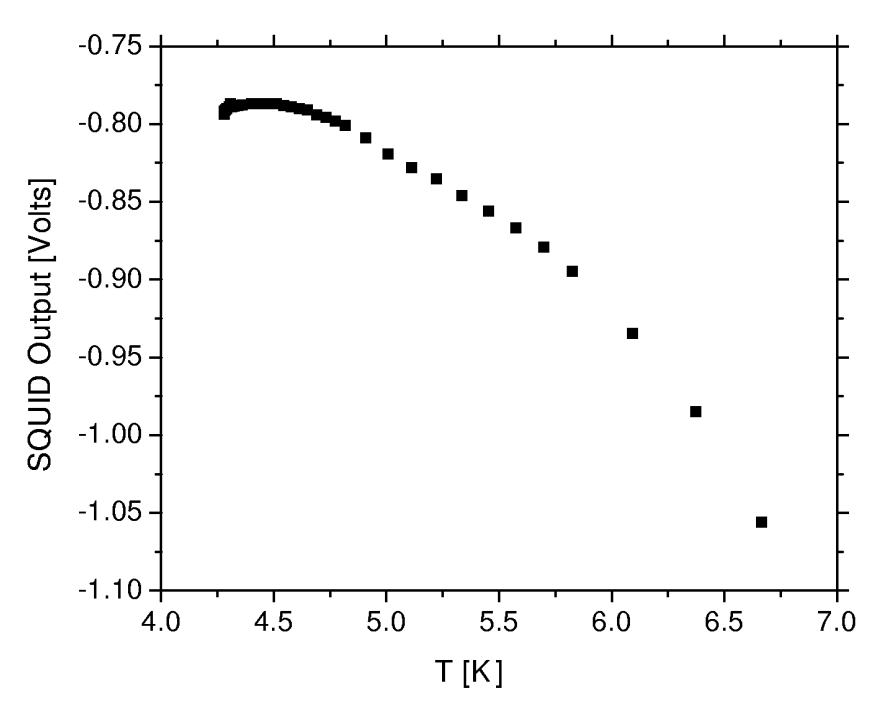
\includegraphics[width=5.7in]{figs/prospective/fig1.ps}
%\caption[Successive vortex avalanches in to \jja.]
%{Successive vortex avalanches into $100\times 150$ \jja\ after initial
%zero field cooling. The color scale has a range of
%$0.09\,\Gauss$ and the length scales are shown in 
%millimeters.
%(a) The array is shown as zero field cooled, in zero external field. 
%(b) The external field has been ramped to $2.4\,\Phinot$ per unit cell.
%(c) The external field has been ramped to $4.8\,\Phinot$ per unit cell.}
%\label{fig:initial_vortex_avalanche}
%\end{figure}

\begin{figure}[p]
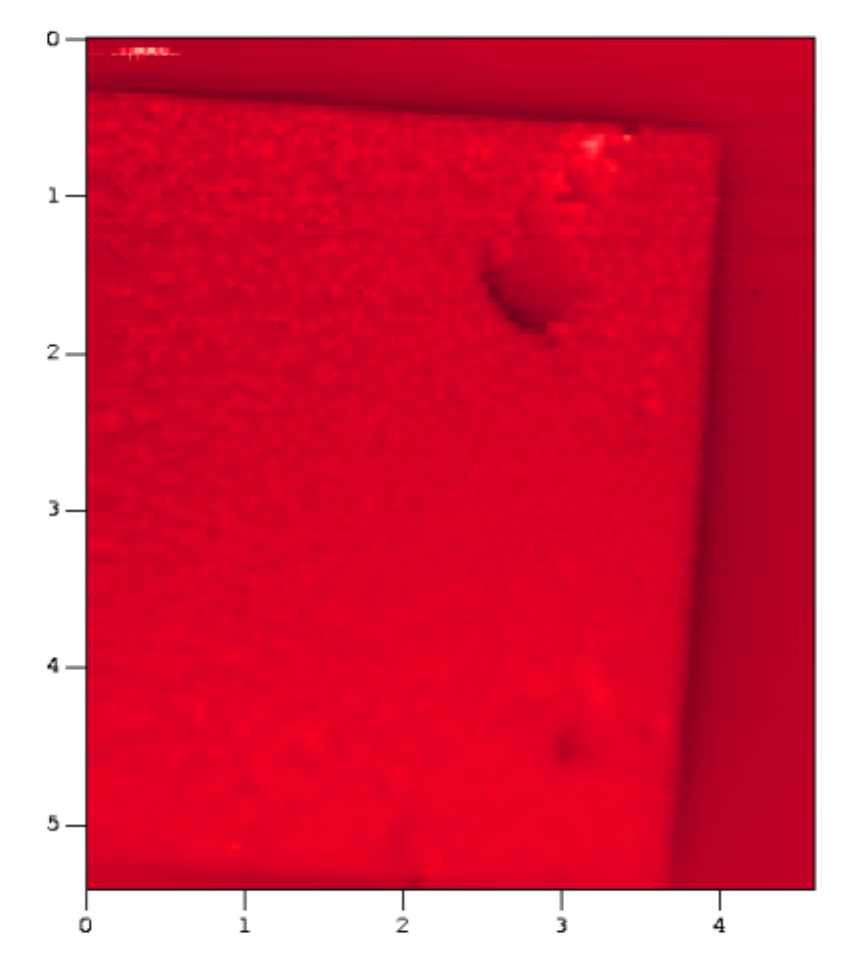
\includegraphics[width=5.7in]{figs/prospective/fig1_a_lg.ps}
\caption[Successive vortex avalanches in to \jja, zero field cooled.]
{Successive vortex avalanches into $100\times 150$ \jja\ after initial
zero field cooling. The color scale has a range of
$0.09\,\Gauss$ and the length scales are shown in 
millimeters.
The array is shown as zero field cooled, in zero external field. 
}
\label{fig:initial_vortex_avalanche_a}
\end{figure}

\begin{figure}[p]
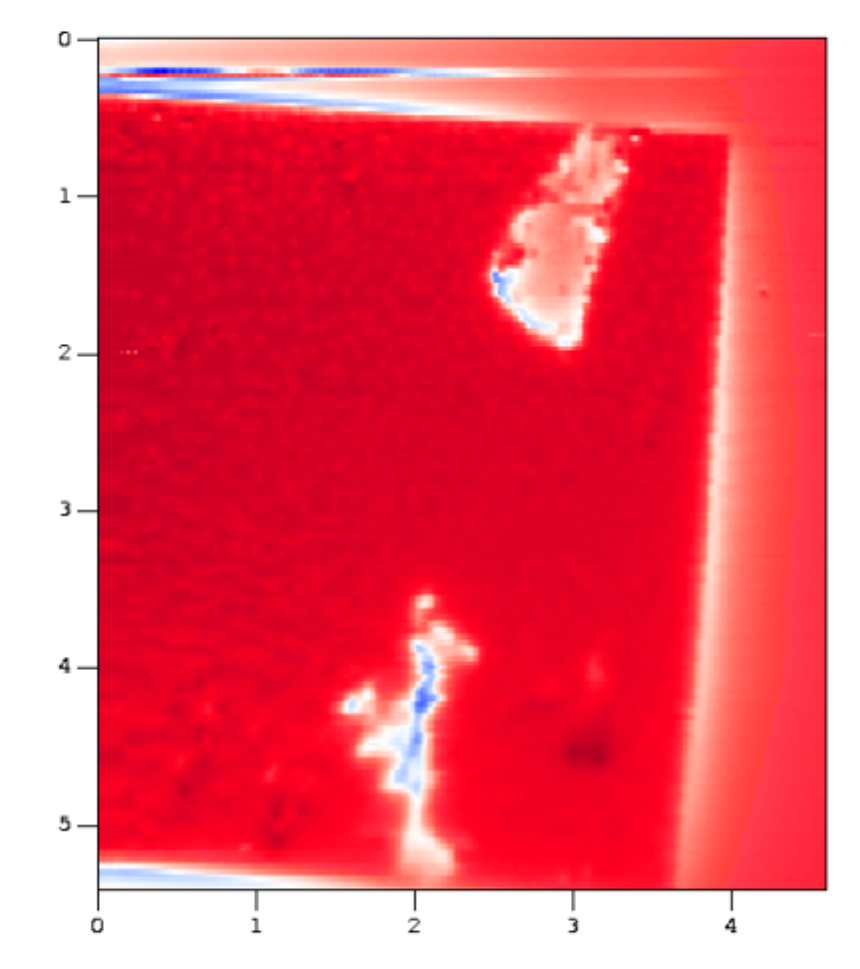
\includegraphics[width=5.7in]{figs/prospective/fig1_b_lg.ps}
\caption[Successive vortex avalanches in to \jja, 
the external field has been ramped to $4.8\,\Phinot$ per unit cell.]
{Successive vortex avalanches into $100\times 150$ \jja\ after initial
zero field cooling. The color scale has a range of
$0.09\,\Gauss$ and the length scales are shown in 
millimeters.
The external field has been ramped to $4.8\,\Phinot$ per unit cell.
}
\label{fig:initial_vortex_avalanche_b}
\end{figure}

\begin{figure}[p]
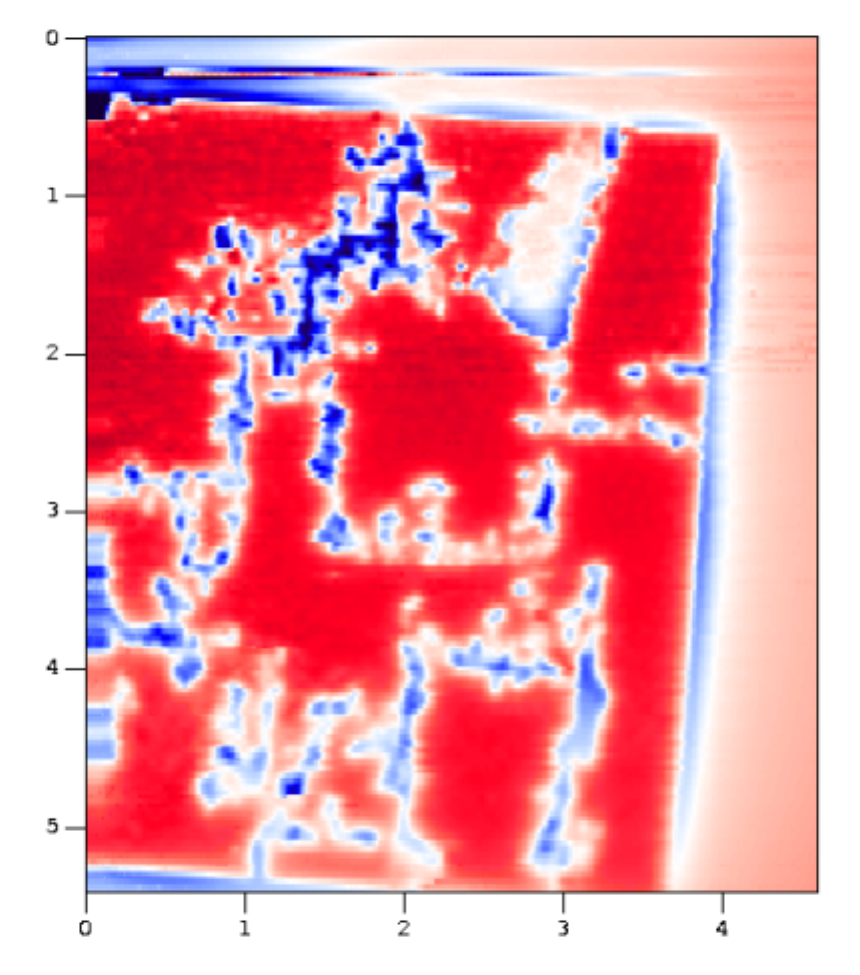
\includegraphics[width=5.7in]{figs/prospective/fig1_c_lg.ps}
\caption[Successive vortex avalanches in to \jja, 
the external field has been ramped to $2.4\,\Phinot$ per unit cell.]
{Successive vortex avalanches into $100\times 150$ \jja\ after initial
zero field cooling. The color scale has a range of
$0.09\,\Gauss$ and the length scales are shown in 
millimeters.
The external field has been ramped to $2.4\,\Phinot$ per unit cell.
}
\label{fig:initial_vortex_avalanche_c}
\end{figure}

%
% fine grained vortex avalanchese
%
%\begin{figure}[p]
%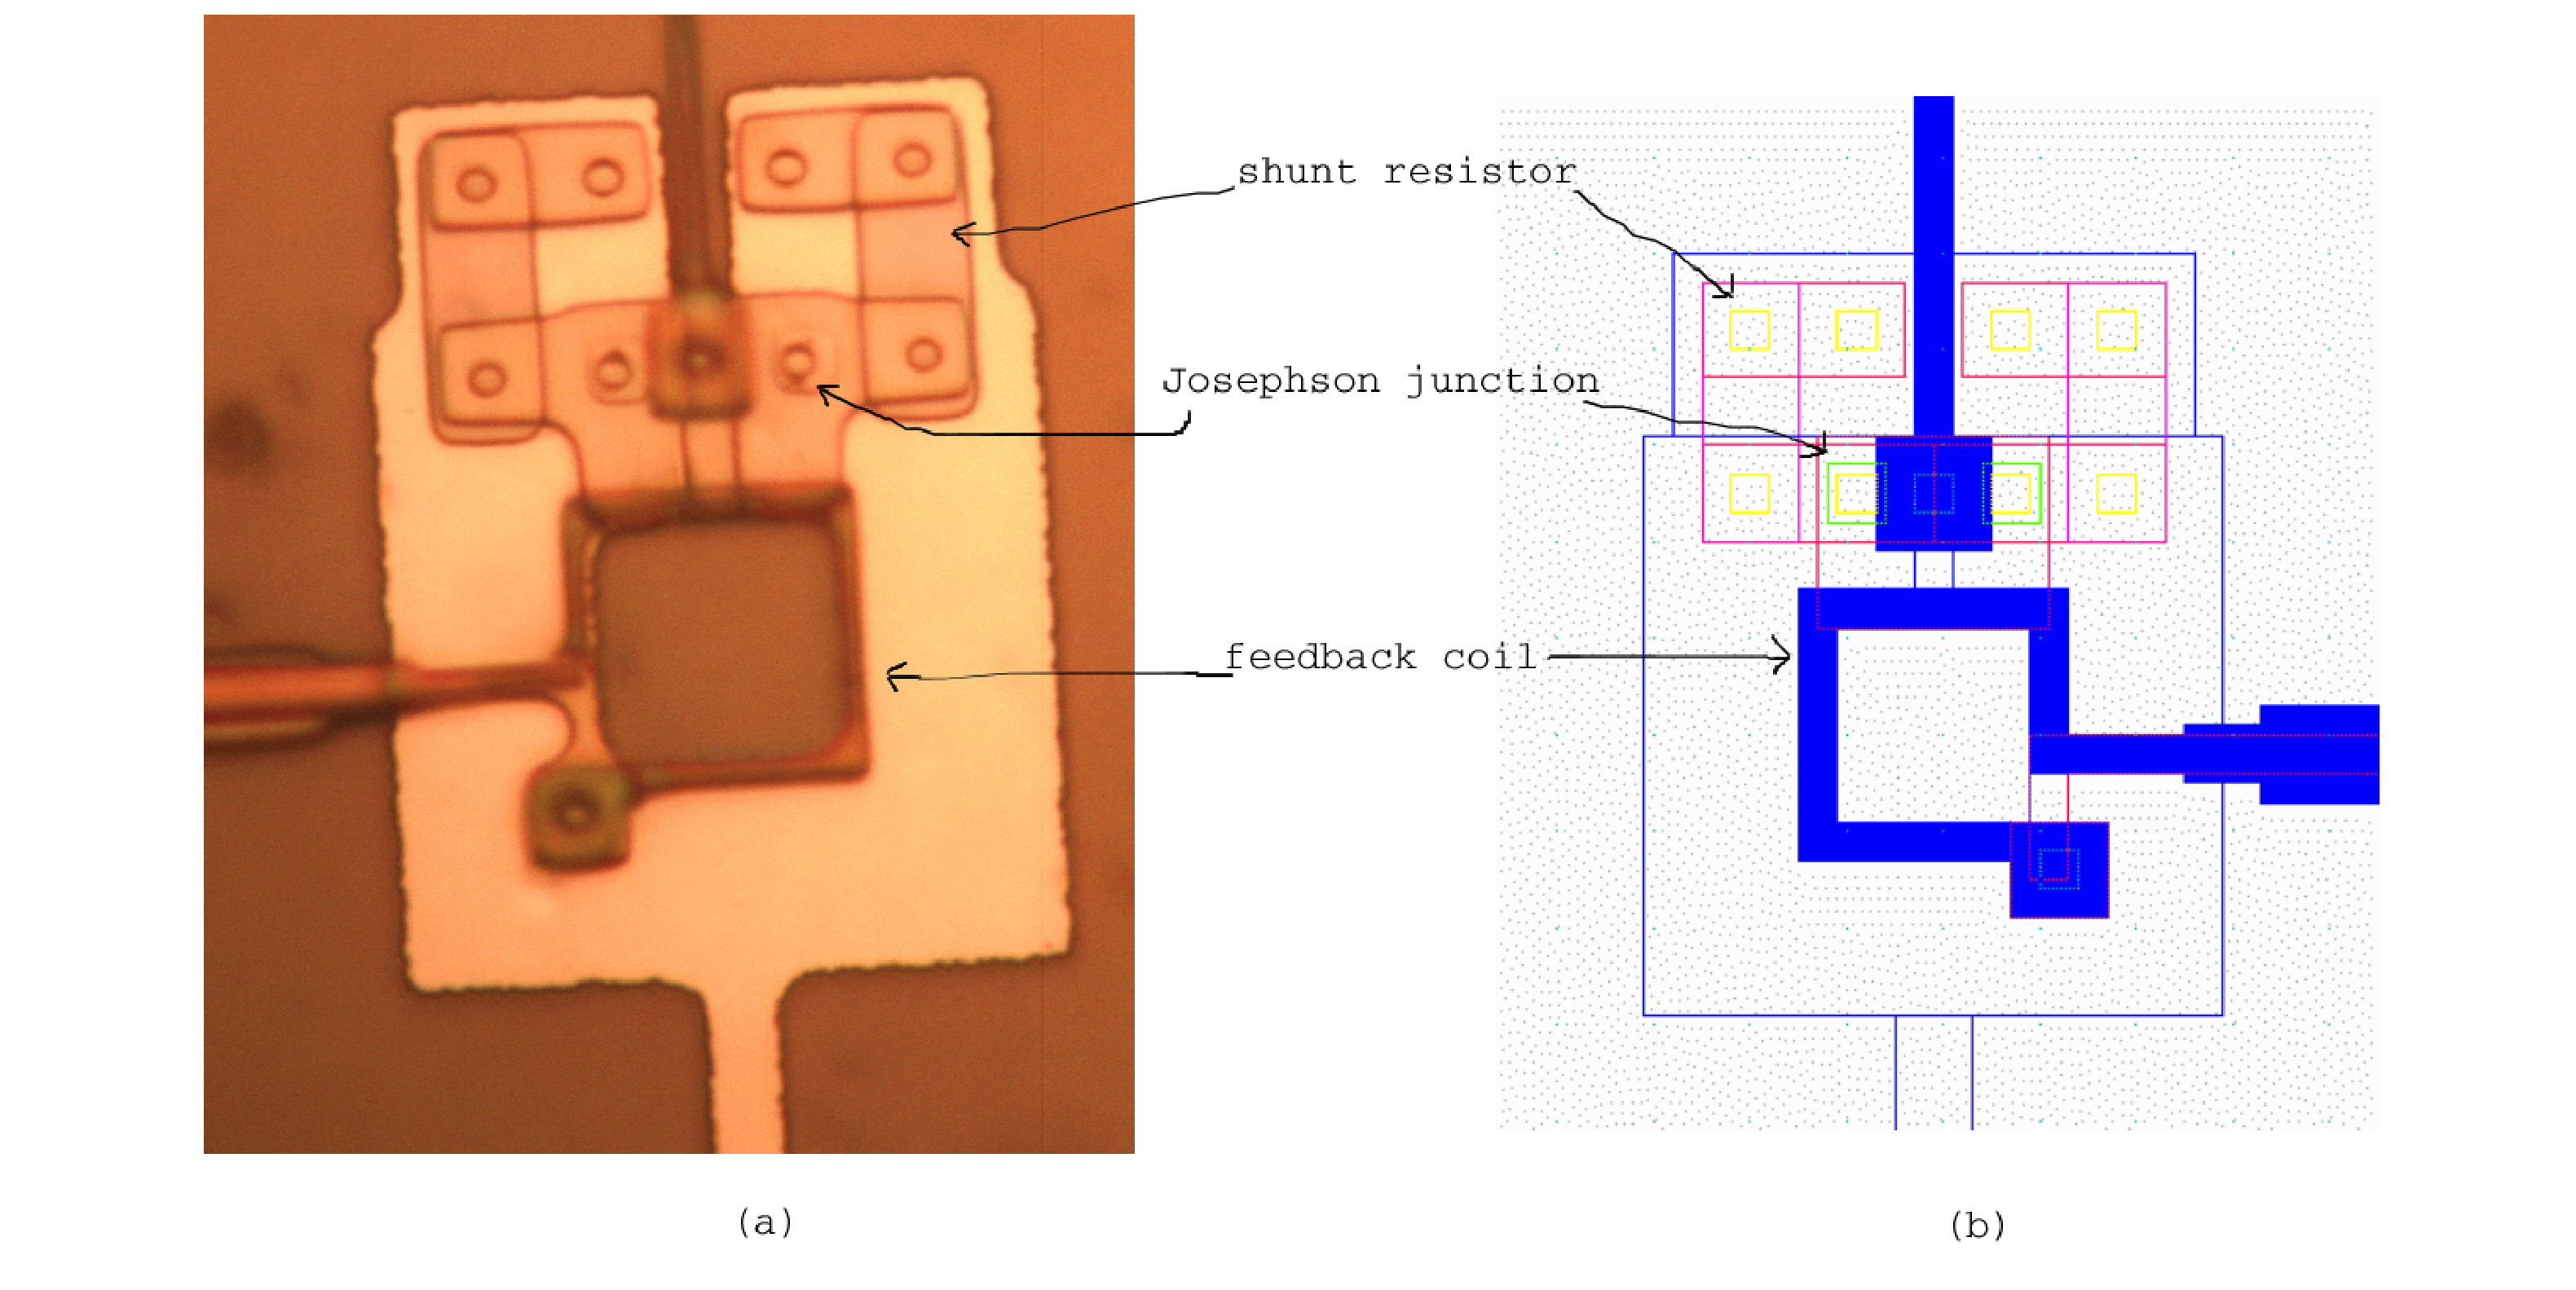
\includegraphics[width=5.7in]{figs/prospective/fig2.ps}
%\caption[Magnetic field images taken between vortex avalanches.]
%{Magnetic field images taken between vortex avalanches. The
%array was zero field cooled, then the external field increased
%to (a) $\Phiext = 2.52\,\Phinot$ per unit cell of the array. 
%(b) $ 2.64\,\Phinot$, numbers corresponding to previous image  
%indicate regions where small scale changes
%occurred in the flux distribution. 
%(c) $ 2.76\,\Phinot$, a second avalanche occurs. 
%For each image, the color scale has a range of
%$0.09\,\Gauss$ and the length scale along the edges is shown in 
%millimeters.
%}
%\label{fig:small_avalanche_steps}
%\end{figure} 

\begin{figure}[p]
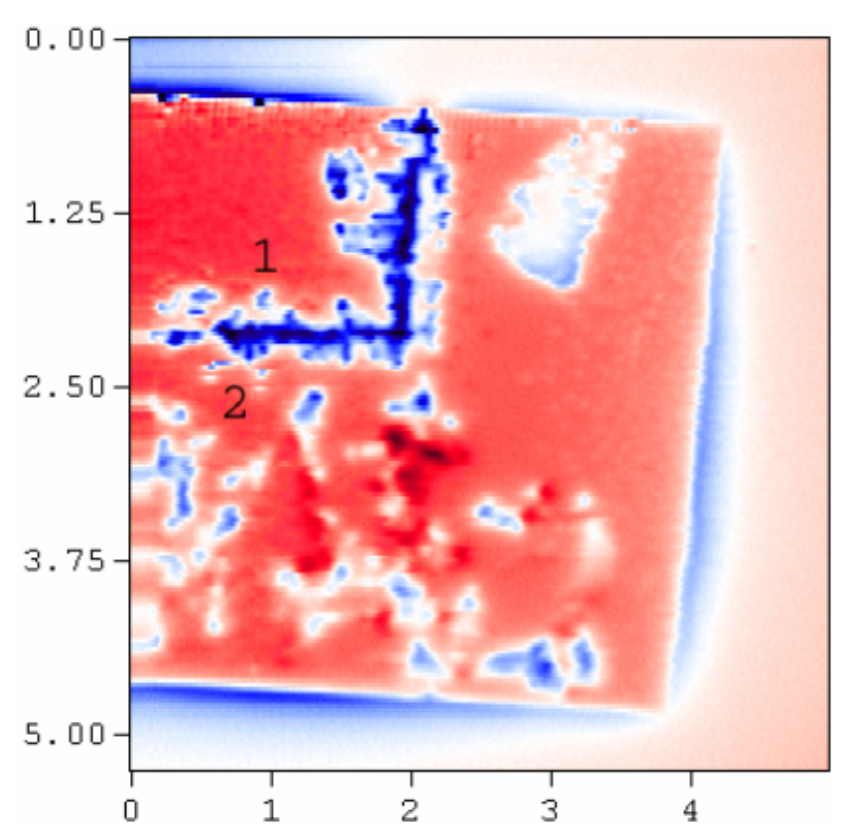
\includegraphics[width=5.7in]{figs/prospective/fig2_a_lg.ps}
\caption[Magnetic field images taken between vortex avalanches, at
$\Phiext = 2.52\,\Phinot$ per unit cell of the array.]
{Magnetic field image taken between vortex avalanches. The
array was zero field cooled, then the external field increased
to  $\Phiext = 2.52\,\Phinot$ per unit cell of the array. 
The color scale has a range of
$0.09\,\Gauss$ and the length scale along the edges is shown in 
millimeters.
}
\label{fig:small_avalanche_steps_a}
\end{figure} 

\begin{figure}[p]
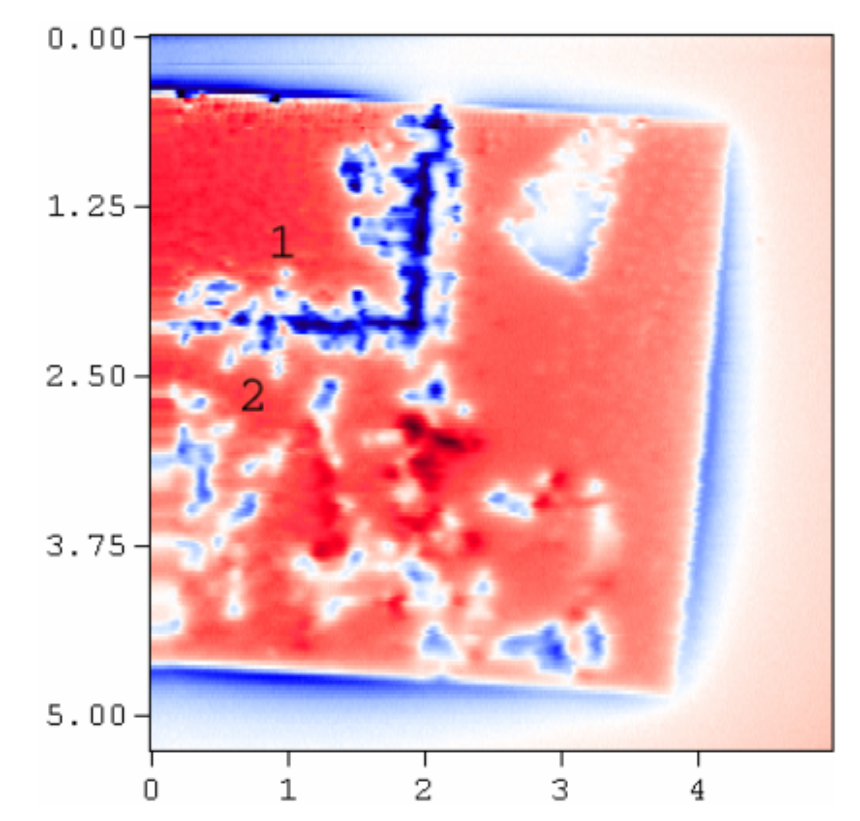
\includegraphics[width=5.7in]{figs/prospective/fig2_b_lg.ps}
\caption[Magnetic field images taken between vortex avalanches, at
$\Phiext = 2.64\,\Phinot$ per unit cell of the array.]
{Magnetic field image taken between vortex avalanches. The
array was zero field cooled, then the external field increased
to  $\Phiext = 2.64\,\Phinot$ per unit cell of the array. 
The color scale has a range of
$0.09\,\Gauss$ and the length scale along the edges is shown in 
millimeters.
}
\label{fig:small_avalanche_steps_b}
\end{figure} 

\begin{figure}[p]
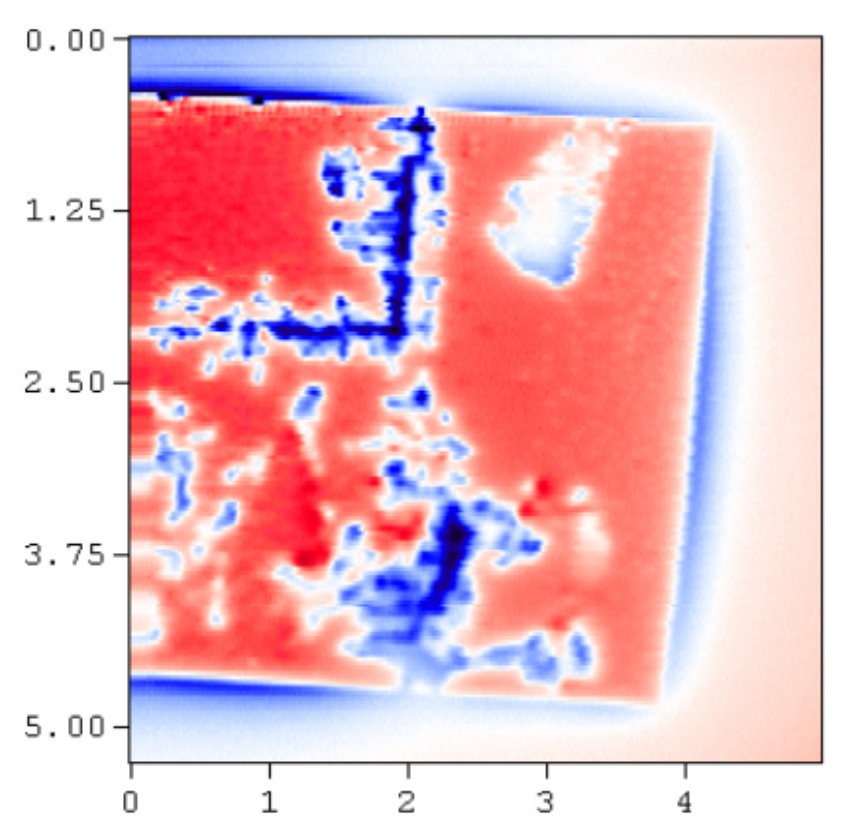
\includegraphics[width=5.7in]{figs/prospective/fig2_c_lg.ps}
\caption[Magnetic field images taken between vortex avalanches, at
$\Phiext = 2.76\,\Phinot$ per unit cell of the array.]
{Magnetic field image taken between vortex avalanches. The
array was zero field cooled, then the external field increased
to  $\Phiext = 2.76\,\Phinot$ per unit cell of the array. 
The color scale has a range of
$0.09\,\Gauss$ and the length scale along the edges is shown in 
millimeters.
}
\label{fig:small_avalanche_steps_c}
\end{figure} 

In order to verify that these avalanches really occurred as avalanches, 
not the aggregation of many small changes
(not visible in our coarse grained steps),
we took fine grained steps in the external field.
At each step we imaged the array
to observe the location of flux in the array. A series of 
these images are shown in \FigRef{fig:small_avalanche_steps_a} through
\FigRef{fig:small_avalanche_steps_c}, in which
the first image \FigRef{fig:small_avalanche_steps_a} 
shows the array immediately after an avalanche at 
$\Phiext = 2.52\,\Phinot$ per unit cell. The second image
\FigRef{fig:small_avalanche_steps_b} shows the array after
the external field was increased to $2.64\,\Phinot$ in which no large
avalanche has occurred, but there have been small redistributions
of flux, particularly at the end of the fingers. The numbers 
in the figure indicate the
regions where this redistribution takes place. 
\FigRef{fig:small_avalanche_steps_c} shows the next avalanche
into the array in an image taken at $2.76\,\Phinot$ per unit cell. 

\FigRef{fig:small_avalanche_steps_b} immediately follows
\FigRef{fig:initial_vortex_avalanche_b} but there are important
distinctions between the two images. We notice that 
\FigRef{fig:small_avalanche_steps_a} is much more complicated 
than \FigRef{fig:initial_vortex_avalanche_b} in which only one small
avalanche has occurred. We can understand this because we have 
increased the external field in \FigRef{fig:small_avalanche_steps_a}
to $\Phiext = 2.52\,\Phinot$ per unit cell versus the external field
in \FigRef{fig:initial_vortex_avalanche_b} of  
$\Phiext = 2.4\,\Phinot$ per unit cell, so we expect further flux
processes to have occurred. 

\subsection{Potential avalanche explanations and further experiments}

\subsubsection{Shunted Josephson-junction arrays}
\index{shunted arrays}

Fernando Araujo-Moreira worked with Paola Barbara looking at AC
susceptibility in shunted and unshunted 
\jjas.\footnote{Refs.
\cite{araujo_prl_78_4625_1997} and \cite{barbara_prb_60_7489_1999}
summarize these results.}
They noticed that there were distinct differences in the AC 
susceptibility between the two cases. In fact, we expect these
differences just by comparing the equations which describe the 
array in both cases. The unshunted array we have already described
(see \EqnRef{eqn:RCSJ}, p.~\pageref{eqn:RCSJ}) 
but in the case of the shunted array, 
we need to modify the equations because of the shunt resistor
which provides a resistive and inductive short around the 
\jjnoun, $R_{s}$ and $L_s$. \FigRef{fig:RCSJ_shunt_schematic}
shows this relationship schematically 
(\cf\ \FigRef{fig:single_junction_sketch}).
The RCSJ model equation becomes modified,
%
\begin{equation}
\label{eqn:RCSJ_shunt_current}
I = I_c \sin(\gamma) + {1\over R} {\Phi_0 \over 2 \pi}{\dif\gamma \over \dif t}
+ C {\Phi_0 \over 2 \pi} {\dif^2\gamma \over \dif t^2} + I_s,
\end{equation}
%
in which $I_s$ is the current through the shunt resistor. To fully define
all of the variables, we now need a further equation which equates the
voltage drops across the junction channel and the shunt channel
%
\begin{equation}
\label{eqn:RCSJ_shunt_volt}
{\Phinot\over 2 \pi} {\dif \gamma \over \dif t} = 
+  L_s {\dif I_s \over \dif t} 
+  I_s R_s 
\end{equation}
%
in which $L$ is the inductance due to the shunt resistor and 
$R_s$ is the resistance of the shunt resistor. However,
if we assume that the inductance is small, we can ignore the induction
term in \EqnRef{eqn:RCSJ_shunt_volt} and the additional resistive term
adds damping to \EqnRef{eqn:RCSJ_shunt_current}. For proper values 
of the shunt resistor, this system becomes \emph{over-damped}.%
\footnote{The distinctions between under-damped and over-damped junctions are discussed
in detail in Tinkham \cite{tinkham} and Newrock 
\etal\,\cite{newrock_ssp_54_263_2000}.}
If we do not neglect the inductance of the shunt resistor, the dynamics
become significantly more complicated, and are discussed in 
detail in Ref.~\cite{cawthorne_jap_84_1126_1998}. 

\begin{figure}[p]
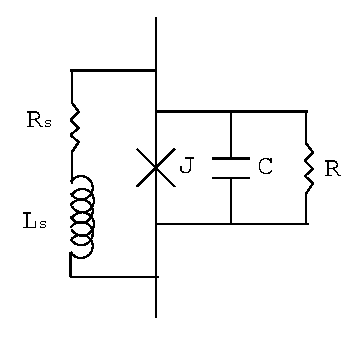
\includegraphics{figs/prospective/shunt_sketch.eps}
\caption[Schematic of shunted \jjnoun.]
{Schematic of shunted \jjnoun. $R_s$ and $L_s$ refer to the 
shunt resistance and inductance respectively. $C$ is the capacitance
of the junction, $R$ refers to the resistive channel through the
junction and $J$ refers to the Josephson supercurrent channel. }
\label{fig:RCSJ_shunt_schematic}
\end{figure}

Once vortices penetrate the shunted array, we may imagine that instead of 
starting a complicated dynamic process by which they move deep into the
array (the fingers) their motion is damped, and penetration takes place 
in a more uniform manner.
Because of these differences between the shunted and unshunted arrays,
we might expect the avalanche behavior to occur only in the 
unshunted array, \ie\ the dynamics causing the avalanches to 
occur would die out in the shunts. This experiment has not 
been attempted, though samples exist with similar parameters to 
the unshunted arrays. 


\subsubsection{Self organized criticality}
\index{self organized criticality}

The flux avalanches into the array look remarkably similar to 
models of self-organized criticality (SOC) \cite{bak_59_381_1987}. 
Several authors have used the SOC model to theoretically describe the critical
state in superconductors
\cite{ginzburg_jetp_79_334_1994,tang_physa_194_315_1993}, and there have
been some measurements of SOC in bulk superconductors
\cite{shi_ieee_5_1721_1995}. A well developed model is that of 
Ginzburg \cite{ginzburg_jetp_79_334_1994} which
says that under a constant drive (\ie\ linearly 
increasing external field) that the flux should enter into the 
array as a form of avalanches. Quantitatively, it describes the 
distribution in physical size of the avalanches, and the distribution
in time between avalanches. SOC says that both of these distributions
must be a power law over many orders of magnitude. 

In order to verify these power law distributions experimentally, 
there are some significant challenges which must be overcome.
To measure the size of the vortex avalanches over a large scale
of avalanche size, we would need to analyze images of about 
$1000$ avalanches or so, which means making SSM images of $1000$
avalanches. For the array size we have been looking at it takes between
one half and one  hour to make the scan. So, to generate the required 
$1000$ images it would take about one month of continuous scanning. 
This amount of scanning is not prohibitive, but would take a considerable
amount of effort and, provided that nothing goes wrong with the 
microscope, can be accomplished. 

Another possibility to verify SOC is to consider the time 
distribution between the avalanches, regardless of avalanche
size. This experiment is not quite as simple to do with the SQUID
microscope, because it requires time resolved, over several decades, 
flux information over the entire
array, which cannot simultaneously be collected while scanning because
of the time required to scan. This experiment could be performed by
putting a gradiometer around the array\footnote{Samples with this 
design have been created, Hypres design \texttt{APN2}.} and 
positioning the SQUID over the secondary coil of the gradiometer to 
measure the changes in flux as the external flux is increased. 
Instead of scanning, the SQUID is positioned in one place and 
a time resolved flux is measured in the SQUID. A similar experiment has 
been performed in bulk samples by Field \etal\,\cite{field_prl_74_1206_1995}
in which they were able to resolve avalanches larger than 
fifty vortices. The SQUID microscope should be able to 
greatly improve on this resolution.


\section{Vortex ratchets}

\index{vortex!ratchet effect}
\index{ratchet effect}
Working with Profs. Steve Rugierro and Laslo Barabasi 
at Notre Dame University, we began
to explore the vortex ratchet effect in superconductors. 
The ratchet effect, as it is 
generally known, first discussed by Feynman
in his lectures \cite{feynmann_lectures},
but has been of particular interest lately in 
superconductors \cite{lee_nature_400_337_1999} and 
\jjas\,\cite{falo_epl_45_700_1999,goldobin_condmat_aug_2000,%
trias_pre_61_2257_2000,wambaugh_prl_83_5106_1999,zapata_prl_77_2292_1996}.
Much of the work surrounding the ratchet effect has been theoretical and 
focused on
understanding just how it is that small (on the scale of Brownian
motion) objects, such as single celled organisms, produce directed
motion
\cite{astumian_science_276_917_1997,astumian_chaos_8_533_1998,%
julicher_rmp_69_1269_1997,magnasco_prl_71_1477_1993}, 
however, there has been some
particularly interesting experimental work, including the chemical
fabrication of molecular scale ratchets \cite{kelly_jorgchem_63_3655_1998}
and micrometer scale AC electric potential ratchets
\cite{prost_prl_72_2652_1994,faucheux_prl_74_1504_1995}.
In a superconductor, we want to use the ratchet effect to 
move vortices around for our benefit, primarily to remove flux
from a superconductor in order to reduce the losses in the 
superconductor when carrying current. 

In order to ratchet vortices around in a superconductor, 
we use the model of Lee \etal\,\cite{lee_nature_400_337_1999}
which 
generates the ratchet potential through the patterning of the 
surface. The line energy of a vortex is
proportional to the length of the vortex in the superconductor
\cite{tinkham} so we can make an asymmetric sawtooth potential
provided that we can pattern the surface of the superconductor
in the shape of this asymmetric sawtooth. The application of an AC
current provides a Lorentz force to the vortices which moves the 
vortices back and forth across the ratchet potential. Since
the ratchet potential is asymmetric the vortices move preferentially
in one direction instead of the other. 

Preliminary samples of niobium with the surface patterned in this way where
fabricated at Notre Dame.\footnote{Samples have been designated
\texttt{RAT1}, \texttt{RAT2} and \texttt{RAT3}. } An Alpha-step%
\cite{kla_tencor} scan, 
in \FigRef{fig:ratchet_alpha_step_a}\ and \FigRef{fig:ratchet_alpha_step_b} 
shows what the surface features
of these samples look like. There are two designs, one with a unidirectional
asymmetric sawtooth, \FigRef{fig:ratchet_alpha_step_b}. This 
sample is designed to move vortices one way across the sample. In principle,
we should be able to see vortices move across this sample. 
The second sample consists of two opposing asymmetric sawtooth ratchets,
\FigRef{fig:ratchet_alpha_step_a}. This sample is designed to flush
vortices away from the center line of the sample and out of the sample. 

%\begin{figure}[p]
%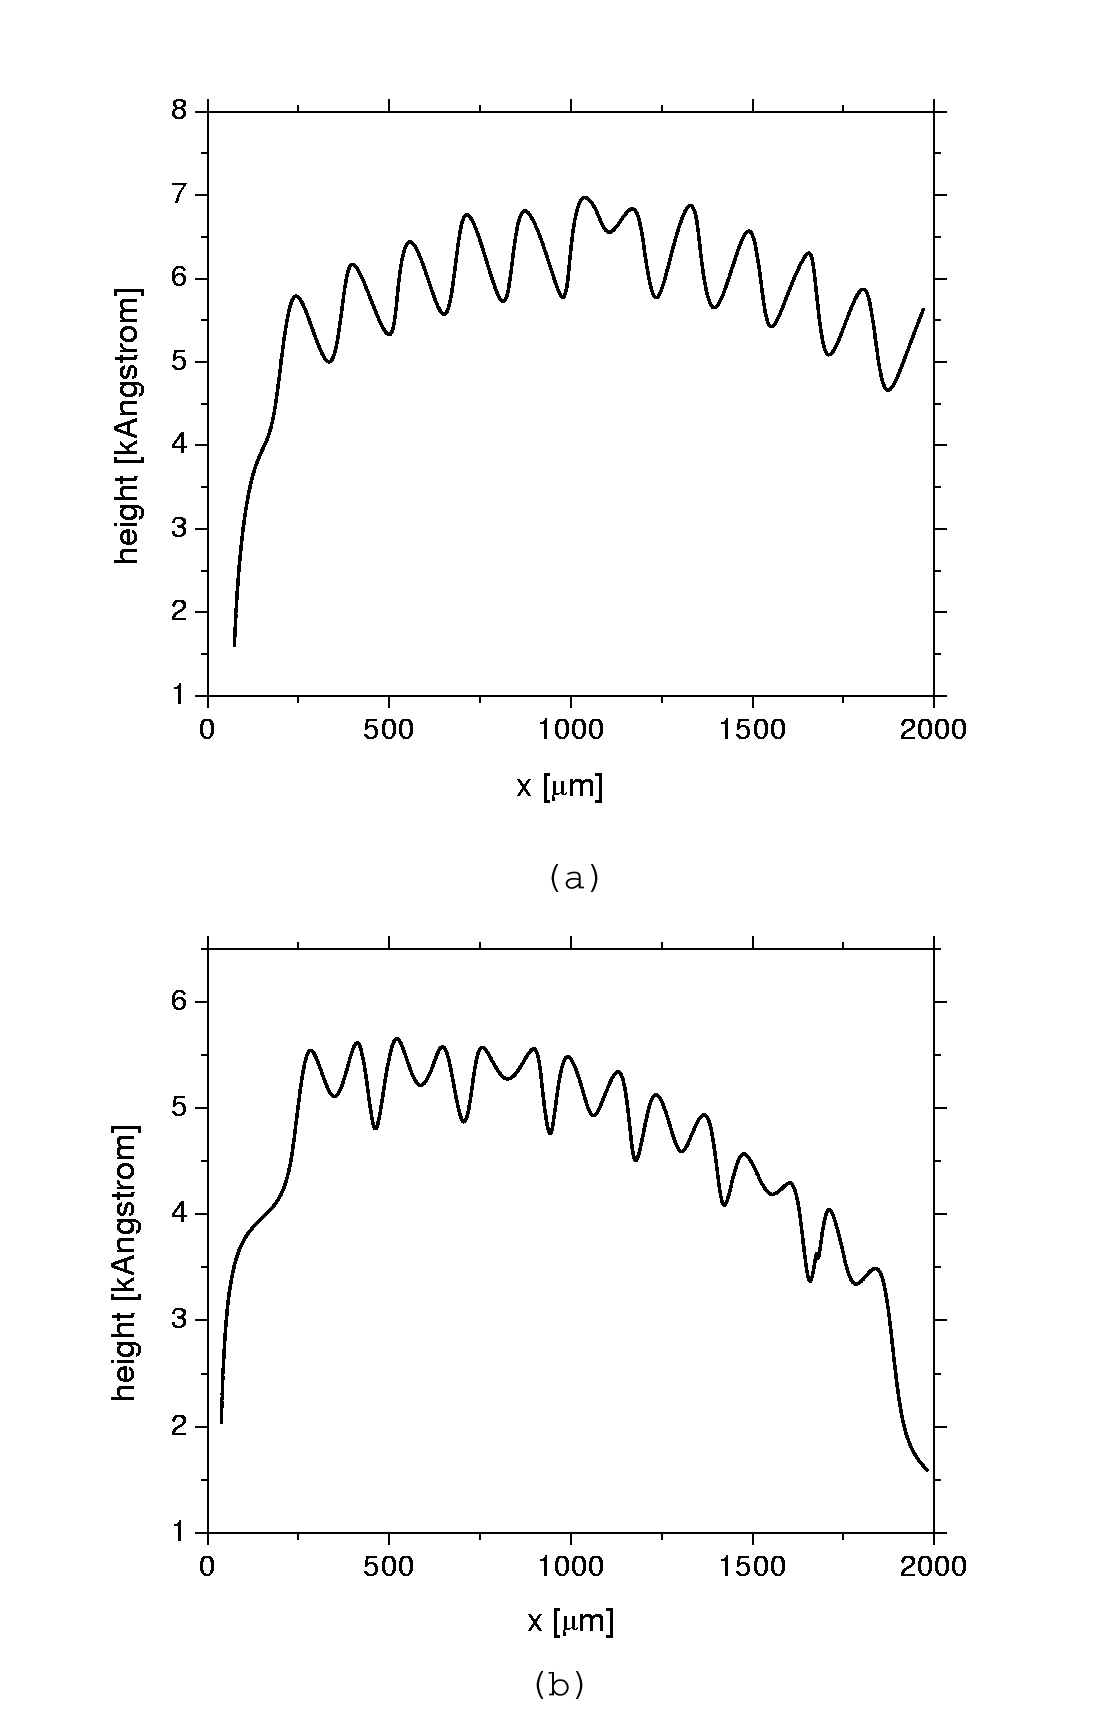
\includegraphics[height=7.0in]{figs/prospective/fig3.ps}
%\caption[Alpha step scan for ratchet samples.]
%{Alpha step scan for ratchet samples. (a) Opposing asymmetric sawtooth
%ratchets. (b) Unidirectional asymmetric sawtooth ratchets. }
%\label{fig:ratchet_alpha_step}
%\end{figure}

\begin{figure}[p]
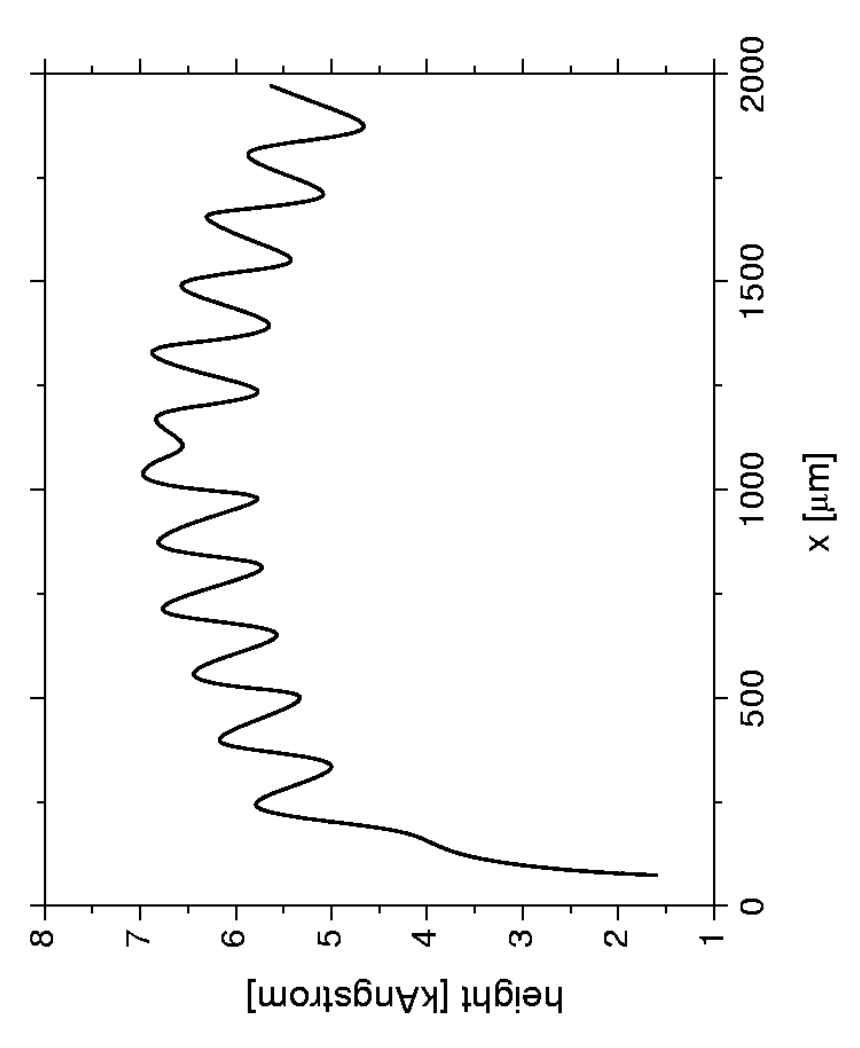
\includegraphics[height=7.0in]{figs/prospective/fig3_a_lg.ps}
\caption{Alpha step scan for ratchet samples. Opposing asymmetric sawtooth
ratchets.}
\label{fig:ratchet_alpha_step_a}
\end{figure}

\begin{figure}[p]
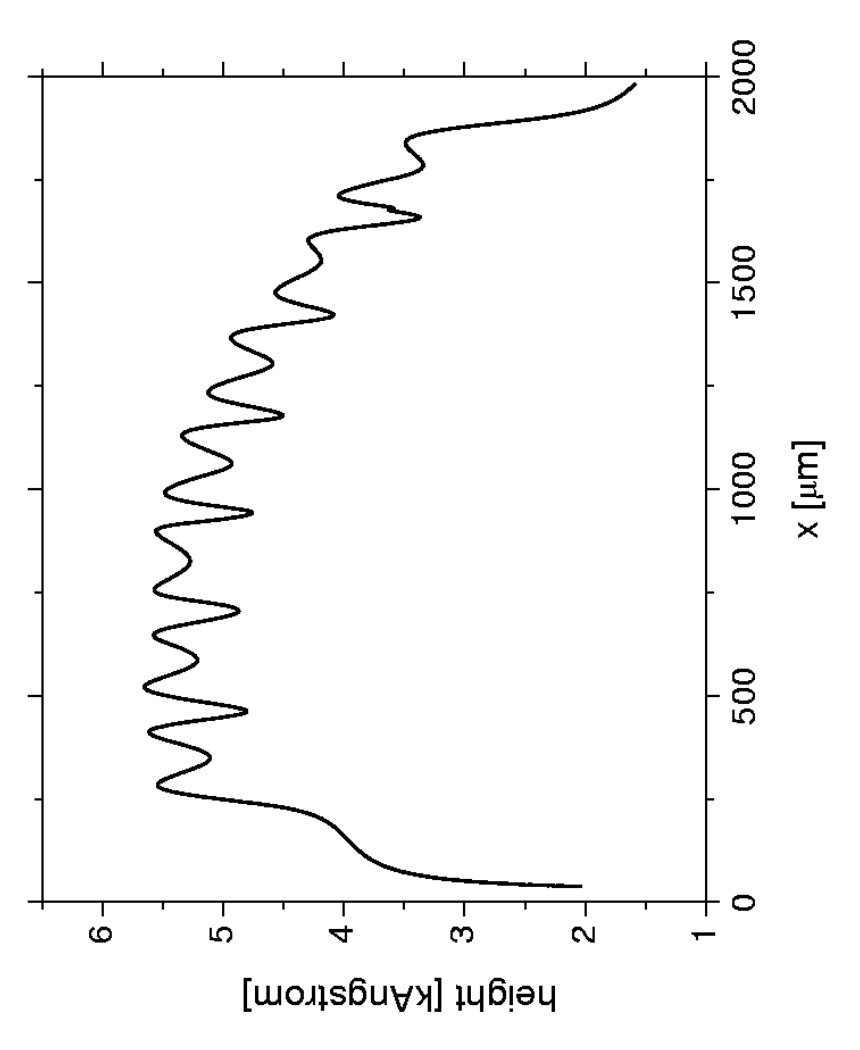
\includegraphics[height=7.0in]{figs/prospective/fig3_b_lg.ps}
\caption{Alpha step scan for ratchet samples.  
Unidirectional asymmetric sawtooth ratchets.}
\label{fig:ratchet_alpha_step_b}
\end{figure}

There are two ways to experimentally look at these samples. Naturally, 
we would want to look at the sample with the SSM and observe the motion
of vortices out of the sample upon application of the AC current. 
Alternatively, we could make current-voltage curves of the samples to 
demonstrate that after flushing vortices out of the sample, the sample
presents lower losses to a supercurrent. 

These samples were placed into our SQUID microscope probe with current
and voltage leads attached for I-V curve measurement. Unfortunately, 
the initial samples had an extremely high critical current, making it
difficult to generate I-V curves, except at temperatures near the
transition temperature of niobium. The problem here is that 
it is difficult to maintain a stable enough temperature in the SQUID probe
to generate reproducible I-V curves. 
Additionally, we attempted to scan these samples before and after
the application of the ratchet current, but were unable to observe
any change within the  samples. 

We believe that in order to observe the ratchet effect in these samples,
we need to have a much lower critical current so that we can observe the 
samples near $4.2\,\kelvin$. At this temperature, the sample will be 
more resistant to small temperature variations. Currently new samples
are being fabricated to meet these requirements and it may soon be
possible to complete this experiment. 
